\chapter{Mejora de la precisión en WR} \label{cap:reloj}

El capítulo anterior ha tratado el sistema desde el punto de vista del 
\textit{firmware}, es decir, la parte en lógica reconfigurable y el 
\textit{software} que se ejecuta en el procesador. Para tener una visión 
completa falta analizar el sistema de relojes encargado de la generación de la 
señal fundamental que mantiene la sincronización en cada dispositivo.

WR consta de un bucle de control, tipo Proporcional Integral (PI), implementado 
en sw y HDL que obtiene la 
diferencia en frecuencia y fase del oscilador local con respecto al del nodo 
maestro. Este bucle de control calcula una serie de valores de consigna cuyo 
objetivo es corregir la frecuencia de oscilación del reloj local para ajustarse 
al maestro. Esto se realiza en la electrónica externa a la FPGA en un sistema 
formado por un conversor digital/analógico (DAC), un oscilador controlado por 
tensión (VCXO) y un \gls{pll}.

\begin{figure}
	\centering
	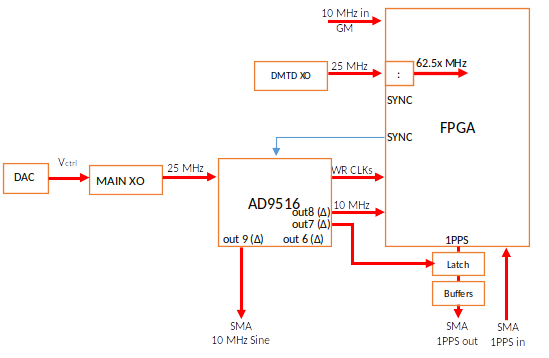
\includegraphics[width=0.7\linewidth]{imagenes/wrclk}
	\caption[Esquema del sistema de reloj en WR]{Esta figura muestra un 
	diagrama de bloques de los componentes principales de la electrónica de 
	relojes para un dispositivo WR.}
	\label{fig:wrclk}
\end{figure}

